% ------------------------------------------------------------------------------
% TYPO3 Version 10.0 - What's New (Serbian Version)
%
% @author	Michael Schams <schams.net>
% @license	Creative Commons BY-NC-SA 3.0
% @link		http://typo3.org/download/release-notes/whats-new/
% @language	Serbian
% ------------------------------------------------------------------------------

\section{Izmene za integratore}
\begin{frame}[fragile]
	\frametitle{Izmene za integratore}

	\begin{center}\huge{Poglavlje 3:}\end{center}
	\begin{center}\huge{\color{typo3darkgrey}\textbf{Izmene za integratore}}\end{center}

\end{frame}

% ------------------------------------------------------------------------------
% TYPO3 Version 10.0 - Breaking Changes

\begin{frame}[fragile]
	\frametitle{Izmene za integratore}
	\framesubtitle{Korenite izmene - Breaking Changes}

	\small
		Integratori obratite pažnju: U TYPO3 v9, deo PHP koda, TSconfig-a, TypoScript
		opcija i uslova, kao i Scheduler tasks-ova je oznacen kao zastareo.

		\vspace{0.2cm}

		U skladu sa TYPO3 \textbf{poilitikom zastarelosti}, ove komponente su izmenjene
		ili uklonjene u TYPO3 v10.0.

		\vspace{0.2cm}

		Ukljucite deprecation log, pažljivo testirajte kod i pregledajte log da locirate
		potencijalne probleme. Koristite ugradjeni
		\href{https://docs.typo3.org/m/typo3/reference-coreapi/master/en-us/ApiOverview/ExtensionScanner/Index.html}{Extension Scanner}
		da dobijete ceo izveštaj o proširenjima koja nisu kompatiblilna.

	\normalsize

\end{frame}

% ------------------------------------------------------------------------------
% Feature | 78432 | Add log message for Switch User action

\begin{frame}[fragile]
	\frametitle{Izmene za integratore}
	\framesubtitle{Promena na drugog korisnika administratorskog interfejsa}

	\begin{itemize}
		\item Log poruka se ispisuje ukoliko se admin korisnik prebaci na drugog korisnika administratorskog interfejsa:
	\end{itemize}

	\begin{figure}
		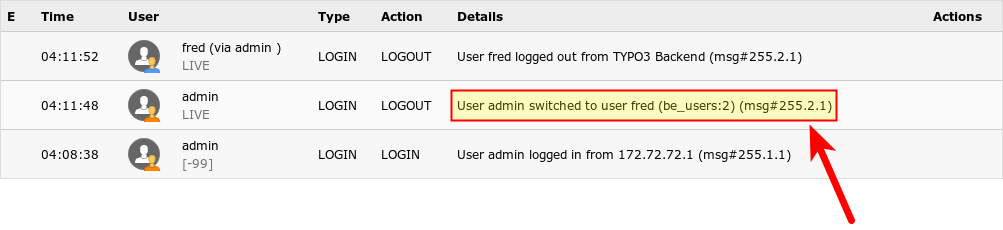
\includegraphics[width=0.90\linewidth]{ChangesForIntegrators/78432-SwitchUserActionLogMessage.png}
	\end{figure}

\end{frame}

% ------------------------------------------------------------------------------
% Feature | 83734 | Add support for current page in configcache
% Breaking | 88564 | PageTSconfig setting TSFE.constants removed
% Breaking | 88657 | Popup configuration in FormEngine dropped

\begin{frame}[fragile]
	\frametitle{Izmene za integratore}
	\framesubtitle{TypoScript izmene}

	\begin{itemize}
		\item TypoScript osobina \texttt{config.cache} sada podržava kljucnu rec
			"\texttt{current}" da bi se odnosila na trenutnu stranu. Na primer:\newline
			\smaller\texttt{config.cache.all = fe\_users:current}\normalsize

		\item Page/User TSconfig podešavanje \texttt{TSFE.constants} je uklonjeno.

			\begin{itemize}\smaller
				\item[\ding{228}] Ukljucite TypoScript uslove u setup/constants i koristite odgovarajucu konfiguraciju u fajlu \texttt{ext\_localconf.php}.
			\end{itemize}

		\item Sledece dve opcije za konfiguraciju velicine popup prozora su uklonjene:

			\begin{itemize}
				\item \texttt{options.popupWindowSize}
				\item \texttt{options.rte.popupWindowSize}
			\end{itemize}

	\end{itemize}

\end{frame}

% ------------------------------------------------------------------------------
% Breaking | 88640 | Database field sys_template.nextLevel and TypoScript sublevel inheritance removed
% Task | 88755 | Remove POST option from typolink.addQueryString

\begin{frame}[fragile]
	\frametitle{Izmene za integratore}
	\framesubtitle{TypoScript izmene}

	\begin{itemize}
		\item Polje u bazi podataka \texttt{nextLevel} u tabeli
			\texttt{sys\_template} je uklonjeno.

			\begin{itemize}\smaller
				\item[\ding{228}] Zamenite ovaj rekord (UID je snimljen u polju \texttt{nextLevel}) sa uslovom da dodate TypoScript za podstrane. Na primer: \texttt{[tree.level > 1]}
			\end{itemize}\normalsize

		\item Sledece vrednosti više \textbf{nisu dozvoljene}:

			\begin{itemize}\smaller
				\item \texttt{typolink.addQueryString.method = POST}
				\item \texttt{typolink.addQueryString.method = GET,POST}
				\item \texttt{typolink.addQueryString.method = POST,GET}
			\end{itemize}\normalsize

			\begin{itemize}\smaller
				\item[\ding{228}] Promenite vrednosti u TypoScript-u, Fluid-u i PHP-u na \texttt{GET}.
			\end{itemize}\normalsize

	\end{itemize}

\end{frame}

% ------------------------------------------------------------------------------
% Breaking | 87583 | Remove obsolete APC Cache Backend implementation
% Breaking | 87558 | Consolidate extbase caches

\begin{frame}[fragile]
	\frametitle{Izmene za integratore}
	\framesubtitle{Keširanje}

	% decrease font size for code listing
	\lstset{basicstyle=\tiny\ttfamily}

	\begin{itemize}
		\item Caching framework više ne podržava \texttt{ApcBackend}

			\begin{itemize}\smaller
				\item[\ding{228}] Koristite umesto toga \textbf{APCu} - obratite pažnju na "u".
			\end{itemize}

\begin{lstlisting}
STARO:
$GLOBALS['TYPO3_CONF_VARS']['SYS']['caching']['cacheConfigurations']['rootline']['backend'] =
\TYPO3\CMS\Core\Cache\Backend\ApcBackend::class;

NOVO:
$GLOBALS['TYPO3_CONF_VARS']['SYS']['caching']['cacheConfigurations']['rootline']['backend'] =
\TYPO3\CMS\Core\Cache\Backend\ApcuBackend::class;
\end{lstlisting}

		\item Extbase keševi \texttt{extbase\_reflection} i \texttt{extbase\_datamapfactory\_datamap}
			su konsolidovani i sada su dostupni kao jedan keš pod nazivom "\texttt{extbase}".

	\end{itemize}

\end{frame}

% ------------------------------------------------------------------------------
% Breaking | 87009 | Use multiple translation files by default in EXT:form

\begin{frame}[fragile]
	\frametitle{Izmene za integratore}
	\framesubtitle{Form Framework}

	% decrease font size for code listing
	\lstset{basicstyle=\tiny\ttfamily}

	\begin{itemize}
		\item Sledeca opcija je preimenovana:\newline
			\small\texttt{translationFile} \textrightarrow\hspace{0.1cm}\texttt{translationFiles}\normalsize
		\item Podrazumevani fajlovi sa prevodima su sada registrovani sa indeksom 10:

			\begin{itemize}
				\item \texttt{EXT:form/Resources/Private/Language/locallang.xlf}
				\item \texttt{EXT:form/Resources/Private/Language/Database.xlf}
			\end{itemize}

		\item Prilagodjene YAML konfiguracije forme treba ažurirati.

\begin{lstlisting}
STARO:
translationFile: path/to/locallang.xlf

NOVO:
translationFiles:
  20: path/to/locallang.xlf
\end{lstlisting}

	\end{itemize}

\end{frame}

% ------------------------------------------------------------------------------
% xxxxx | Cache Storage Type

\begin{frame}[fragile]
	\frametitle{Izmene za integratore}
	\framesubtitle{Cache Storage Type (1)}

	\begin{itemize}

		\item TYPO3 poseduje fleksibilan sistem keširanja sa podrazumevanim podešavanjima
			i ovo je idealno za vecinu slucajeva.

		\item Tip skladišta se sada može podesiti da se fino podesiti keš i povecaju
			performanse u zavisnosti od okruženja

			\begin{itemize}
				\item Izaberite \textbf{database} skladište za standardna okruženja ili ako se
				 	koristi network file system (NFS).
				\item Izaberite \textbf{file system} ako se koristi sistem sa podeljenim
					bazama podataka

				\item Izaberite \textbf{custom cache settings} da podesite skladište za svaki
					keš posebno.
			\end{itemize}

		\item Za kompleksnije instalacije treba uzeti u obzir memory-based keš kao što je
			\href{https://redis.io/}{Redis}
			ili
			\href{https://memcached.org/}{Memcached}.


	\end{itemize}

\end{frame}

% ------------------------------------------------------------------------------
% xxxxx | Cache Storage Type

\begin{frame}[fragile]
	\frametitle{Izmene za integratore}
	\framesubtitle{Cache Storage Type (2)}

	\begin{itemize}

		\item Administratorski interfejs: \textbf{MAINTENANCE} \ding{223}\hspace{0.1cm}\textbf{Settings} \ding{223}\hspace{0.1cm}\textbf{Cache}:
		\end{itemize}

	\begin{figure}
		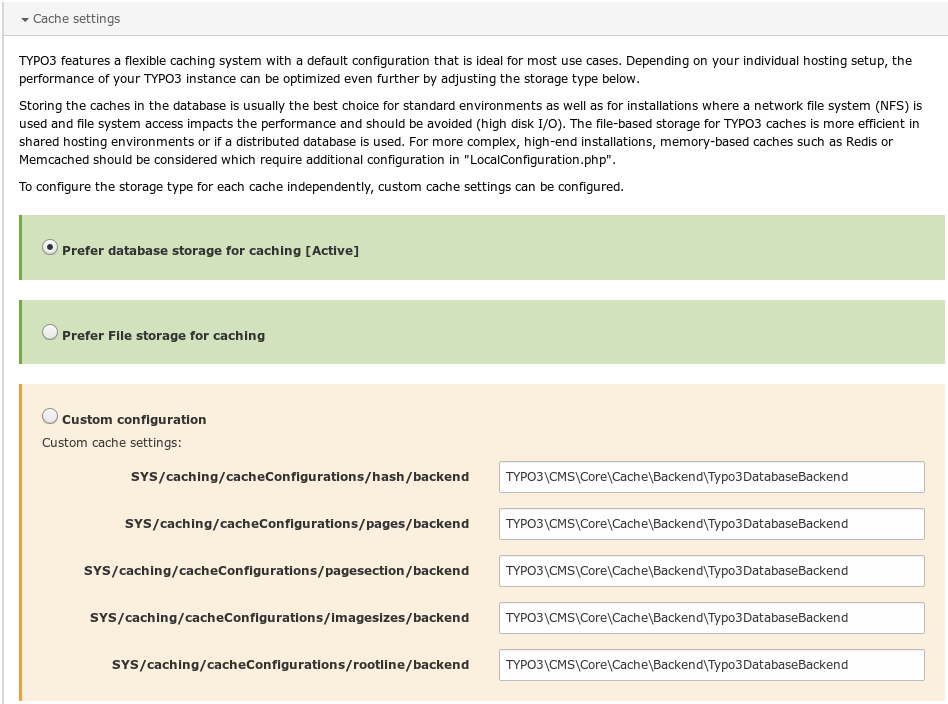
\includegraphics[width=0.60\linewidth]{ChangesForIntegrators/xxxxx-CacheStorageType.png}
	\end{figure}

\end{frame}

% ------------------------------------------------------------------------------
% 87499 | Drop extensions "taskcenter" and "sys_action" from core

\begin{frame}[fragile]
	\frametitle{Izmene za integratore}
	\framesubtitle{Task Center i \texttt{EXT:sys\_action}}

	\begin{itemize}

		\item Sistemska proširenja \texttt{EXT:taskcenter} i \texttt{EXT:sys\_action}
			su uklonjena iz jezgra aplikacije.

		\item Sada postoje kao posebna proširenja dostupna u
			\href{https://extensions.typo3.org/}{TER}
			i
			\href{https://github.com/FriendsOfTYPO3}{GitHub}.

		\item Obratite pažnju na
			\href{https://typo3.org/community/teams/typo3-development/initiatives/typo3-dashboard-initiative/}{Dashboard Initiative}
			za novi i bolji pristup.

	\end{itemize}

\end{frame}

% ------------------------------------------------------------------------------
% Feature | 88648 | Define Twitter Card Type In Page Properties
% Important | 86577 | Query parameters are now included in canonicalized URLs

\begin{frame}[fragile]
	\frametitle{Izmene za integratore}
	\framesubtitle{Razno}

	% decrease font size for code listing
	\lstset{basicstyle=\tiny\ttfamily}

	\begin{itemize}

		\item Tip Twitter karte se sada moze izabrati/prilagoditi.
			Ova opcija generiše meta tag \texttt{twitter:card} na korisnickom interfejsu.

\begin{lstlisting}
page {
  meta {
    twitter:card = summary_large_image
    twitter:card.replace = 1
  }
}
\end{lstlisting}

		\item Samo neophodni parametri za izracunavanje cHash-a su ukljuceni u kanonicnim URL-ovima po podrazumevanim podešavanjima.
			Dodatni parametri upita se sada mogu podešavati:

\begin{lstlisting}
$GLOBALS['TYPO3_CONF_VARS']['FE']['additionalCanonicalizedUrlParameters'].
\end{lstlisting}

		\smaller
			Napomena: dodajte samo parametre koji menjaju sadržaj strane. U suprotnom pretraživaci ce oznaciti Vaše strane kao dupliran sadržaj.
		\normalsize

	\end{itemize}

\end{frame}

% ------------------------------------------------------------------------------
% Breaking | 88681 | Import Of PHP Files In Import Export Files Removed
% Breaking | 88500 | RTE image handling functionality dropped
% Breaking | 81950 | Remove leftover workspaces unpublishing functionality

\begin{frame}[fragile]
	\frametitle{Izmene za integratore}
	\framesubtitle{Razno}

	% decrease font size for code listing
	\lstset{basicstyle=\tiny\ttfamily}

	\begin{itemize}

		\item Kada uvozite XML podatke korišcenjem \texttt{EXT:impexp}, File Deny Pattern se sada primenjuje
			i odbacuje, na primer, ugradjene PHP fajlove.


		\item RTE funkcionalnost za upravljanje slikama je kompletno uklonjena.
			Za podršku za slike u CKEditor-u, možete da koristite na primer \texttt{EXT:rte\_ckeditor\_image}.

		\item Osobina u workspaces za \textit{unpublishing} rekorda je uklonjena u v10
			(ukljucujuci i polje u bazi podataka \texttt{sys\_workspace.unpublish\_time}).
			Ova funkcionalnost je onemogucena u TYPO3 v4.5 i nije korišcena ili omogucemna od strane TYPO3.

	\end{itemize}

\end{frame}

% ------------------------------------------------------------------------------
% Breaking | 88772 | JavaScript script tags omit type=text/javascript in HTML5
% Remove system extension EXT:rsaauth
% Remove system extension EXT:fe_edit

\begin{frame}[fragile]
	\frametitle{Izmene za integratore}
	\framesubtitle{Razno}

	% decrease font size for code listing
	\lstset{basicstyle=\tiny\ttfamily}

	\begin{itemize}

		\item Kada se generiše HTML5, \texttt{<script>} tagovi više ne sadrže atribut
			\texttt{type="text/javascript"}.

		\item Ovo može da se omoguci korišcenjem TypoScript-a ako je neophodno:

\begin{lstlisting}
page {
  includeJS {
    myfile = EXT:example/Resources/Public/JavaScript/myfile.js
    myfile.type = text/javascript
  }
}
\end{lstlisting}

		\item Uklonjena su sledeca zastarela sistemska proširenja:

			\begin{itemize}
				\item \texttt{EXT:rsaauth}
				\item \texttt{EXT:fe\_edit}
			\end{itemize}

	\end{itemize}

\end{frame}

% ------------------------------------------------------------------------------
